\subsection{Docker}
\label{sec:analysis:docker}

Докер — это открытая платформа для разработки, доставки и эксплуатации приложений. Docker разработан для более быстрого выкладывания ваших приложений. С помощью docker вы можете отделить ваше приложение от вашей инфраструктуры и обращаться с инфраструктурой как управляемым приложением. Docker помогает выкладывать ваш код быстрее, быстрее тестировать, быстрее выкладывать приложения и уменьшить время между написанием кода и запуска кода. Docker делает это с помощью легковесной платформы контейнерной виртуализации, используя процессы и утилиты, которые помогают управлять и выкладывать ваши приложения.

В своем ядре docker позволяет запускать практически любое приложение, безопасно изолированное в контейнере. Безопасная изоляция позволяет вам 
запускать на одном хосте много контейнеров одновременно. Легковесная природа контейнера, который запускается без дополнительной нагрузки гипервизора, позволяет вам добиваться больше от вашего железа.

Платформа и средства контейнерной виртуализации могут быть полезны в следующих случаях:
упаковывание вашего приложения (и так же используемых компонент) в docker контейнеры;
раздача и доставка этих контейнеров вашим командам для разработки и тестирования;
выкладывания этих контейнеров на ваши продакшены, как в дата центры так и в облака.

Docker прекрасно подходит для организации цикла разработки. Docker позволяет разработчикам использовать локальные контейнеры с приложениями и сервисами. Что в последствии позволяет интегрироваться с процессом постоянной интеграции и выкладывания (continuous integration and deployment workflow).

Например, ваши разработчики пишут код локально и делятся своим стеком разработки (набором docker образов) с коллегами. Когда они готовы, отравляют код и контейнеры на тестовую площадку и запускают любые необходимые тесты. С тестовой площадки они могут оправить код и образы на продакшен

Основанная на контейнерах docker платформа позволят легко портировать вашу полезную нагрузку. Docker контейнеры могут работать на вашей локальной машине, как реальной так и на виртуальной машине в дата центре, так и в облаке.

Портируемость и легковесная природа docker позволяет легко динамически управлять вашей нагрузкой. Вы можете использовать docker, чтобы развернуть или погасить ваше приложение или сервисы. Скорость docker позволяет делать это почти в режиме реального времени.

\begin{figure}[h!]
\centering
	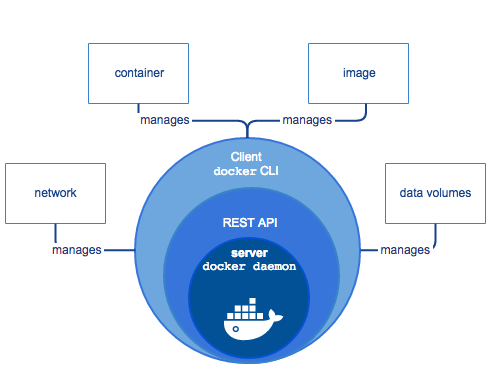
\includegraphics[scale=0.7]{components-flow.png}
	\caption{Конь}
\end{figure}
\clearpage

Docker легковесен и быстр. Он предоставляет устойчивую, рентабельную альтернативу виртуальным машинам на основе гипервизора. Он особенно полезен в условиях высоких нагрузок, например, при создания собственного облака или платформа-как-сервис (platform-as-service). Но он так же полезен для маленьких и средних приложений, когда вам хочется получать больше из имеющихся ресурсов.

Docker состоит из двух главных компонент:

\begin{itemize}
  \item docker: платформа виртуализации с открытым кодом;
  \item docker Hub: наша платформа-как-сервис для распространения и управления docker контейнерами;
\end{itemize}
